\documentclass[a4paper,12pt,titlepage]{article}
\usepackage{amsmath} 
\usepackage{amssymb}
\usepackage{color}
\usepackage[nottoc]{tocbibind}
\usepackage{mathrsfs}
\usepackage{float}
\usepackage{indentfirst}
\author{\textit{Jiang Yicheng}\\\textit{515370910224}}
\title{\textbf{VE203\\
		Assignment 8}}
\date{\today}
\usepackage{dsfont}
\usepackage[top=1in, bottom=1in, left= 1in, right=1in]{geometry}
\usepackage{fancyhdr,lastpage}
	\pagestyle{fancy}
	\fancyhf{}
\cfoot{Page \thepage\ of \pageref{LastPage}}
\usepackage{multirow}
\usepackage{gauss}
\usepackage[colorlinks=true,linkcolor=black]{hyperref}
\usepackage[linesnumbered,ruled,longend]{algorithm2e}
\SetKwInOut{Input}{Input}
\SetKwInOut{Output}{Output}
\newcommand{\To}{\KwTo}
\newcommand{\Ret}{\KwRet}
\SetKwProg{Fn}{Function}{\string:}{end}
\SetKwFunction{mc}{MC}
\newcommand{\udots}{\mathinner{\mskip1mu\raise1pt\vbox{\kern7pt\hbox{.}}\mskip2mu\raise4pt\hbox{.}\mskip2mu\raise7pt\hbox{.}\mskip1mu}}
\SetKwFunction{pow}{PowMod}
\usepackage{graphicx}
\usepackage{extarrows}
\begin{document}

\maketitle

\section*{Exercise 8.1} 
$19-A,17-T,14-C,20-K,23-P,18-E,19-A,8-R,12-L,16-H,3-B,21-O,25-D,6-M,15-S,22-V,11-N$
So the message is
$$ATTACK\,\,\,PEARL\,\,\,HARBOR\,\,\,DECEMBER\,\,\,SEVEN$$
\section*{Exercise 8.2} 
$n=p\cdot q=7\cdot 11=77,e=7,m=23$, so
$$c\equiv m^e\equiv 23^7\equiv23\cdot(-10)^3\equiv (-10)\cdot 23\cdot23\equiv 100\equiv23\,\,(mod\,\,77)$$
So the number $m=23$ is encrypted as $c=23$.
\section*{Exercise 8.3}
Since $(G,\circ)$ is cyclic $g$ is a generator of $G$, then $(G,\circ)$ is group already and $\forall x\in G,\exists k\in \mathbb{N},g^k=x$.

$\forall x,y\in G$, we can set $x=g^{k_1},y=g^{k_2}$, then 
$$x\circ y=g^{k_1}\circ g^{k_2}=\underbrace{g\circ g\circ\cdots\circ g}_{k_1+k_2\,\,\,times}=g^{k_2}\circ g^{k_2}=y\circ x$$
so the group $(G,\circ)$ satisfies community. So $(G,\circ)$ is abelian.
\section*{Exercise 8.4}
According to the question, we can set that
$$3^{a}\equiv 6\,\,(mod\,\,7),3^{b}\equiv 5\,\,(mod\,\,7)$$
and we can find that
$$3^5\equiv 4\cdot3\equiv5\,\,(mod\,\,7), 3^3\equiv6\,\,(mod\,\,7),3^6\equiv 5\cdot 3\equiv1\,\,(mod\,\,7)$$
so $a=3,b=5$ and $3^{ab}=3^{15}$.

So their common secret key is $3^{15}$.


\section*{Exercise 8.5}

\subsection*{i)}
\begin{figure}[H]
    \centering
    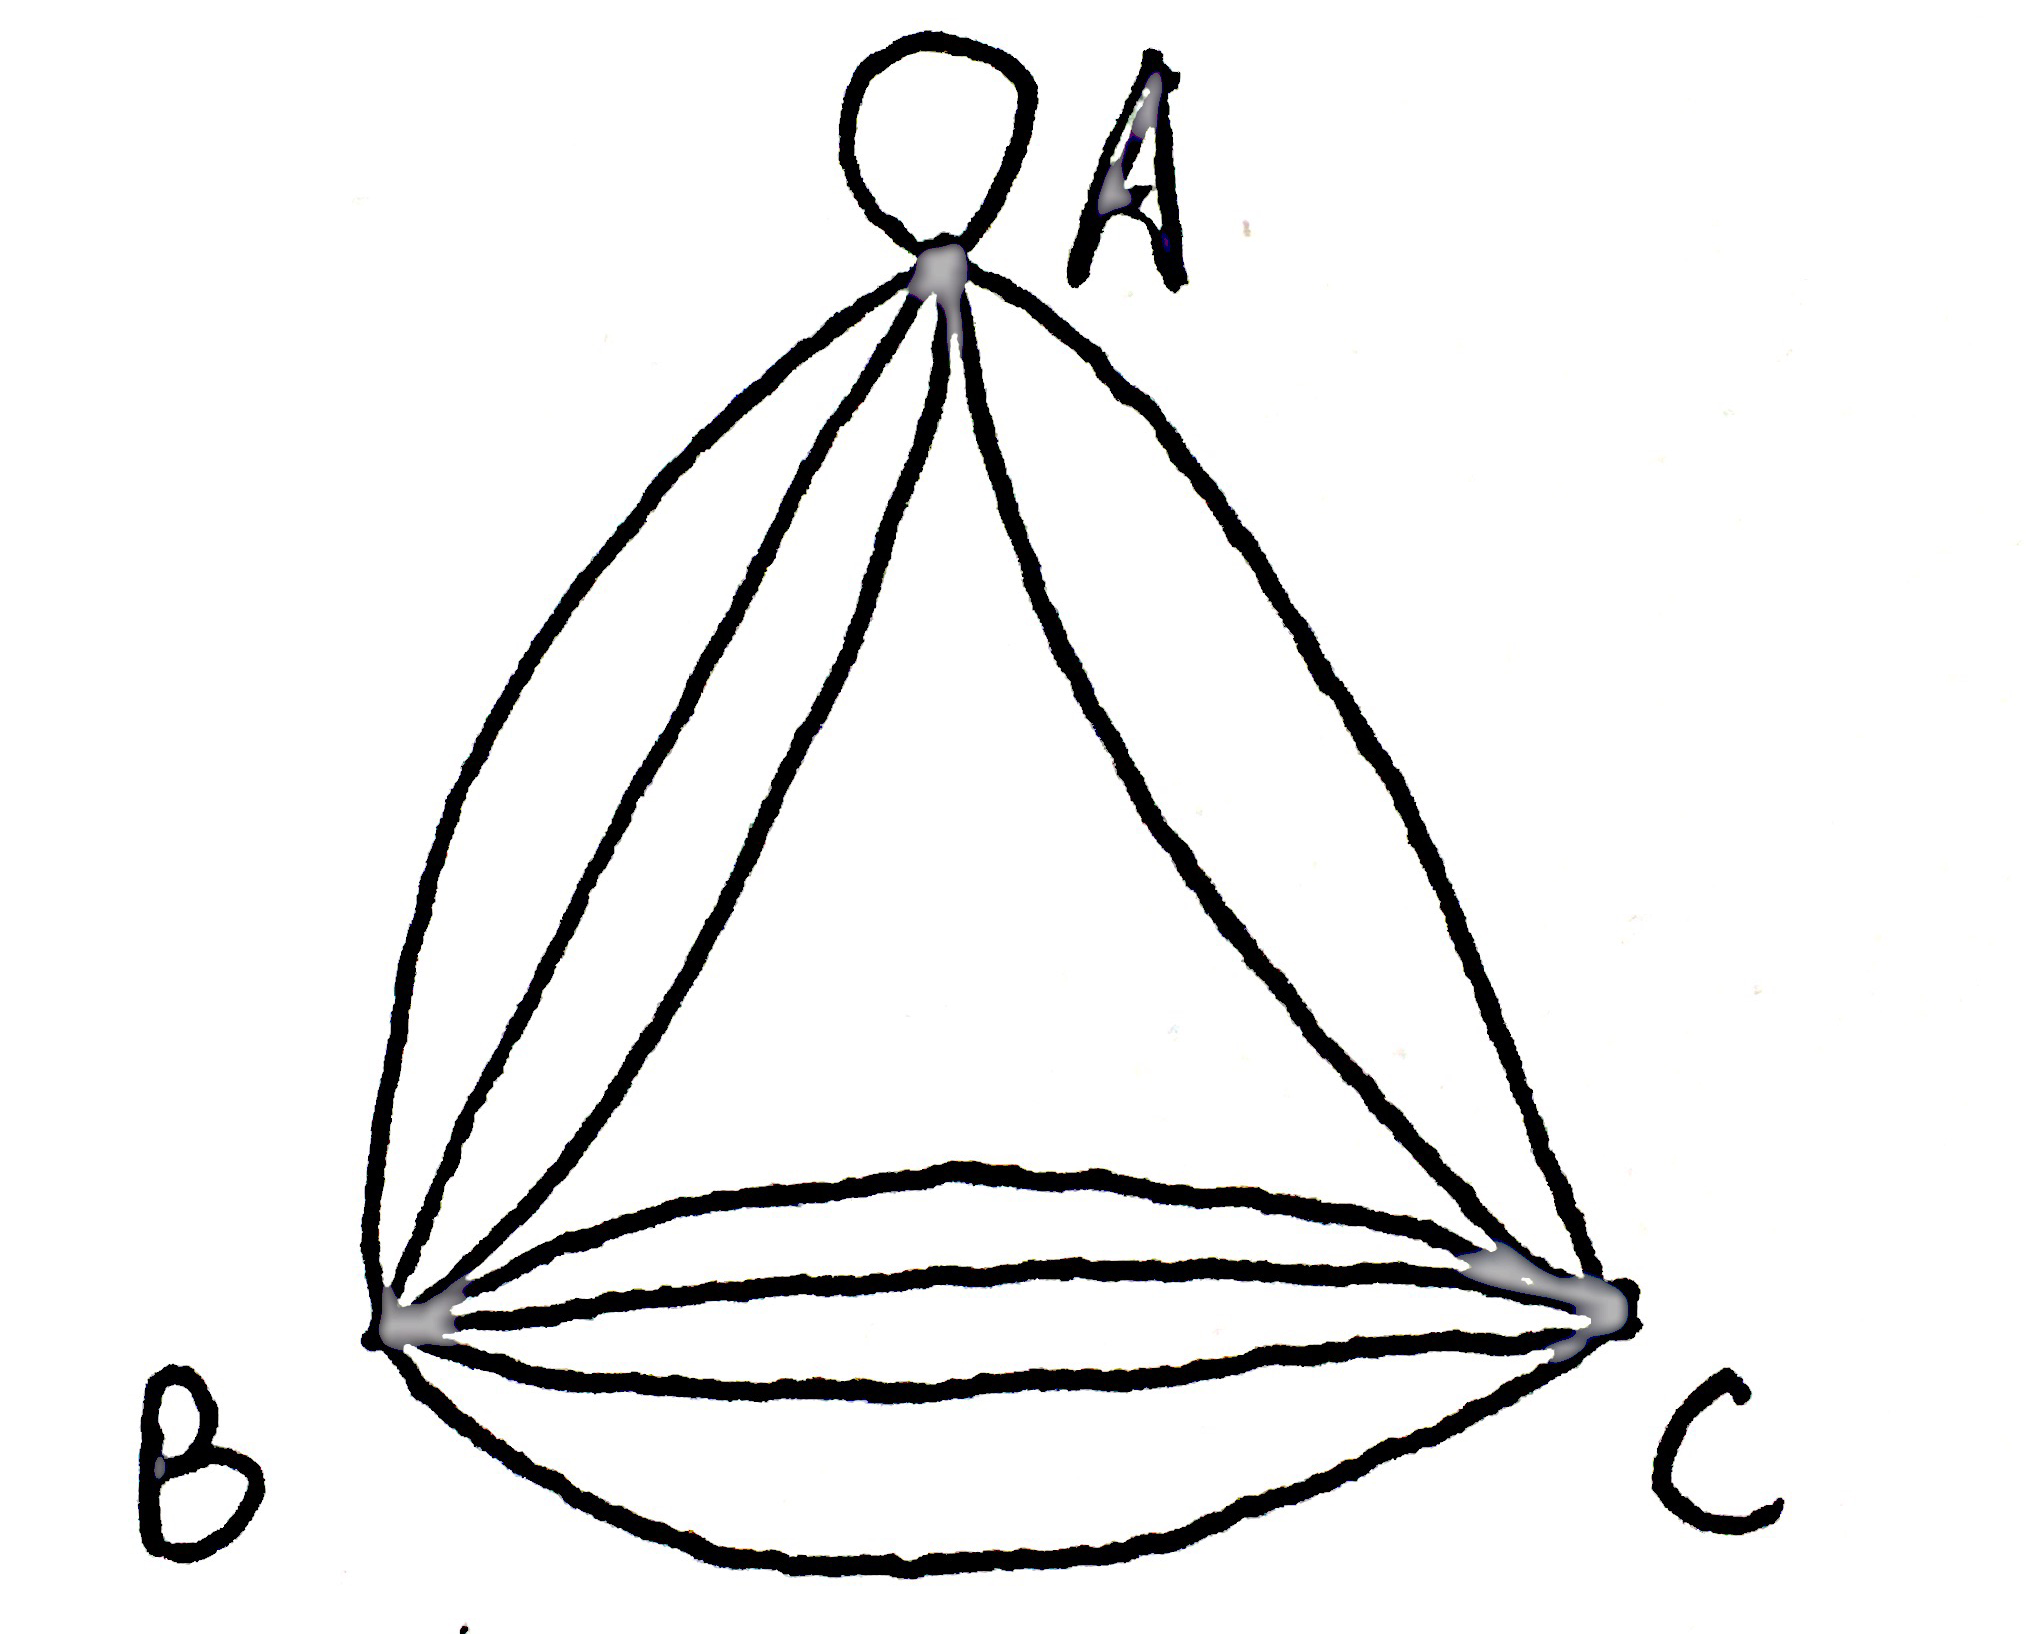
\includegraphics[width=6cm]{1.png}
\end{figure}
\begin{enumerate}
\item The number of vertices: 6
\item The number of edges: 6
\item $deg(a_1)=2,deg(a_2)=4,deg(a_3)=1,deg(a_4)=3,deg(a_5)=2,deg(a_6)=0$
\item Isolated vertices: $a_6$
\item Pendant vertices: $a_3$
\item It is a simple graph.
\item The adjacency matrix is
\begin{equation*} 
A_G=\begin{array}{c}
\\
a_1\\
a_2\\
a_3\\
a_4\\
a_5\\
a_6
\end{array} 
\begin{array}{c}   
    a_1\,\,\, a_2 \,\, a_3 \,\, a_4 \,\, a_5 \,\, a_6 \\
  \left(                 
  \begin{array}{cccccc}   
    0 & 1 & 0 & 1 & 0 & 0\\  
    1 & 0 & 1 & 1 & 1 & 0\\
    0 & 1 & 0 & 0 & 0 & 0\\
    1 & 1 & 0 & 0 & 1 & 0\\
    0 & 1 & 0 & 1 & 0 & 0\\
    0 & 0 & 0 & 0 & 0 & 0\\
  \end{array}
\right)  
\end{array}   
\end{equation*}
\end{enumerate}


\subsection*{ii)}
\begin{figure}[H]
    \centering
    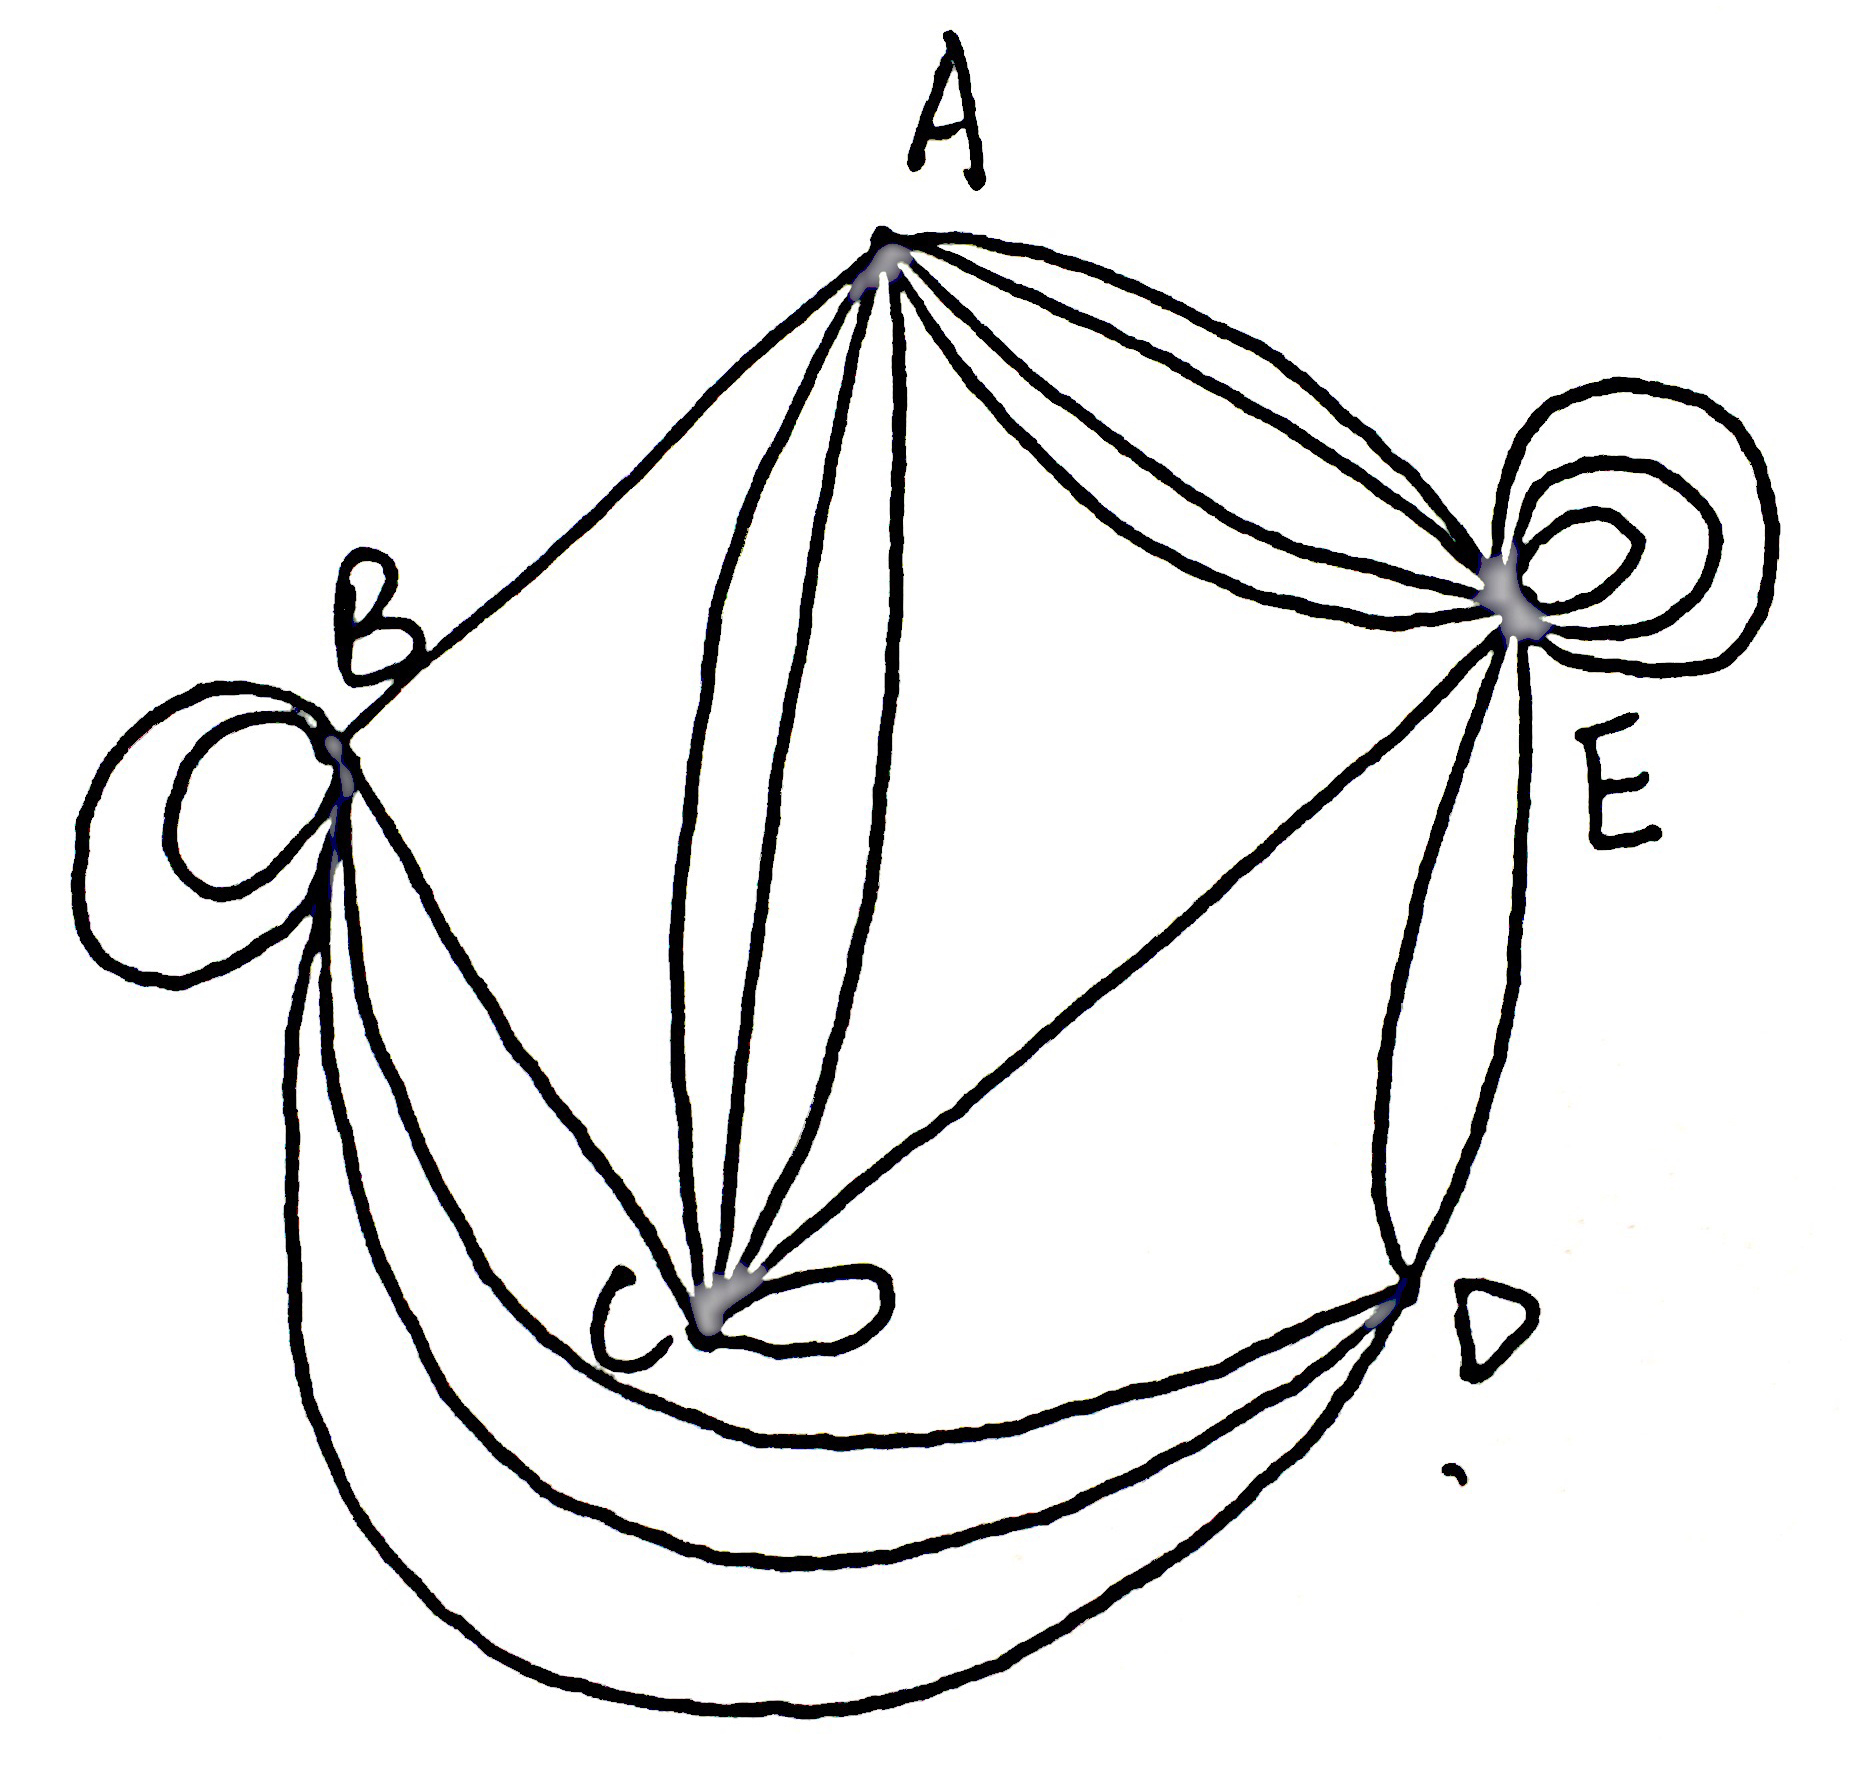
\includegraphics[width=6cm]{2.png}
\end{figure}
\begin{enumerate}
\item The number of vertices: 6
\item The number of edges: 12
\item $deg(a_1)=6,deg(a_2)=5,deg(a_3)=0,deg(a_4)=3,deg(a_5)=5,deg(a_6)=5$

\item Isolated vertices: $a_3$
\item Pendant vertices: no
\item It is a multigraph and also a pseudograph.
\item The adjacency matrix is
\begin{equation*} 
A_G=\begin{array}{c}
\\
a_1\\
a_2\\
a_3\\
a_4\\
a_5\\
a_6
\end{array} 
\begin{array}{c}   
    a_1\,\,\, a_2 \,\, a_3 \,\, a_4 \,\, a_5 \,\, a_6 \\
  \left(                 
  \begin{array}{cccccc}   
    1 & 1 & 0 & 1 & 0 & 0\\  
    1 & 0 & 0 & 1 & 1 & 0\\
    0 & 0 & 0 & 0 & 0 & 0\\
    1 & 1 & 0 & 0 & 1 & 0\\
    0 & 1 & 0 & 1 & 0 & 1\\
    0 & 0 & 0 & 0 & 1 & 1\\
  \end{array}
\right)  
\end{array}   
\end{equation*}
\end{enumerate}


\subsection*{iii)}
\begin{figure}[H]
    \centering
    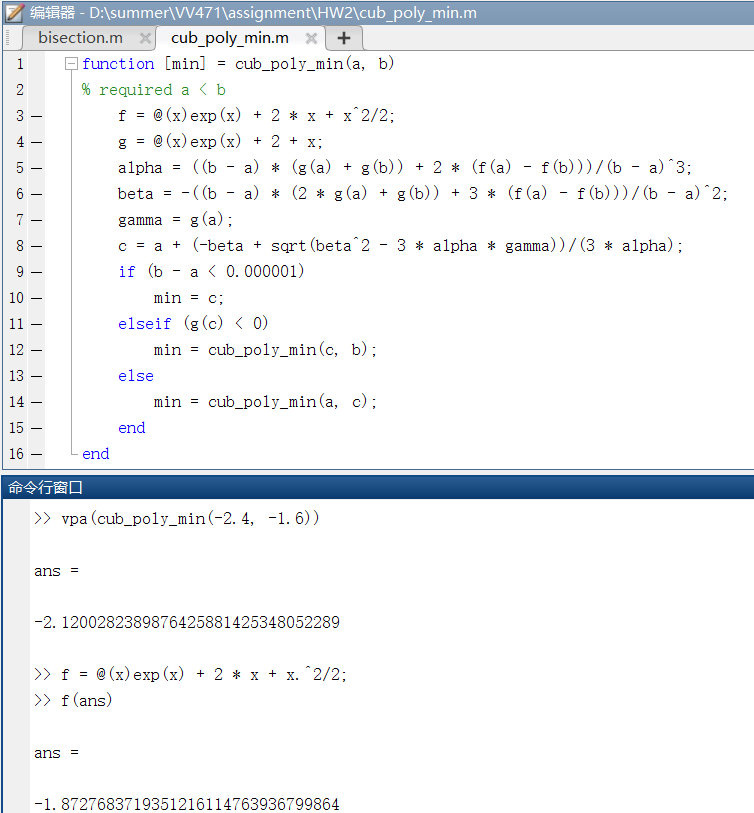
\includegraphics[width=6cm]{3.png}
\end{figure}
\begin{enumerate}
\item The number of vertices: 9
\item The number of edges: 10
\item $deg(a_1)=2,deg(a_2)=2,deg(a_3)=2,deg(a_4)=0,deg(a_5)=0,
deg(a_6)=3,\\deg(a_7)=2,deg(a_8)=4,deg(a_9)=5$

\item Isolated vertices: $a_4,a_5$
\item Pendant vertices: no
\item It is a multigraph.
\item The adjacency matrix is
\begin{equation*} 
A_G=\begin{array}{c}
\\
a_1\\
a_2\\
a_3\\
a_4\\
a_5\\
a_6\\
a_7\\
a_8\\
a_9
\end{array} 
\begin{array}{c}   
    a_1\,\, a_2 \,\,\, a_3 \,\, a_4 \,\, a_5 \,\, a_6\,\, a_7\,\, a_8\,\,\, a_9 \\
  \left(                 
  \begin{array}{ccccccccc}   
    0 & 0 & 0 & 0 & 0 & 1 & 0 & 0 & 1\\  
    0 & 0 & 0 & 0 & 0 & 0 & 1 & 0 & 1\\
    0 & 0 & 0 & 0 & 0 & 1 & 0 & 1 & 0\\
    0 & 0 & 0 & 0 & 0 & 0 & 0 & 0 & 0\\
    0 & 0 & 0 & 0 & 0 & 0 & 0 & 0 & 0\\
    1 & 0 & 1 & 0 & 0 & 0 & 1 & 0 & 0\\
    0 & 1 & 0 & 0 & 0 & 1 & 0 & 0 & 0\\
    0 & 0 & 1 & 0 & 0 & 0 & 0 & 0 & 1\\
    1 & 1 & 0 & 0 & 0 & 0 & 0 & 1 & 0\\
  \end{array}
\right)  
\end{array}   
\end{equation*}
\end{enumerate}
\section*{Exercise 8.6}
\subsection*{i)}
\begin{figure}[H]
    \centering
    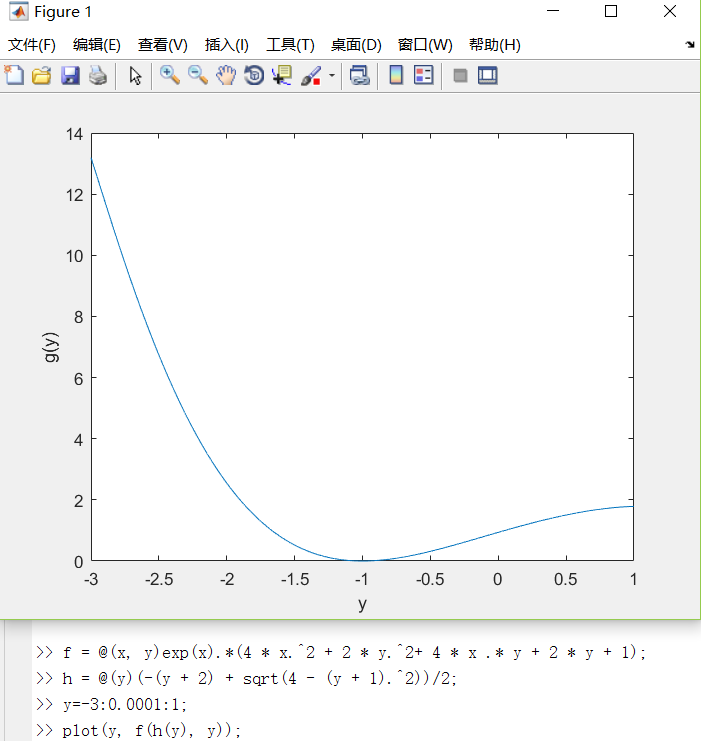
\includegraphics[width=6cm]{4.png}
\end{figure}
This graph is bipartite and a bipartition of it is $(\lbrace a,c\rbrace,\lbrace b,d,e\rbrace)$

\subsection*{ii)}
\begin{figure}[H]
    \centering
    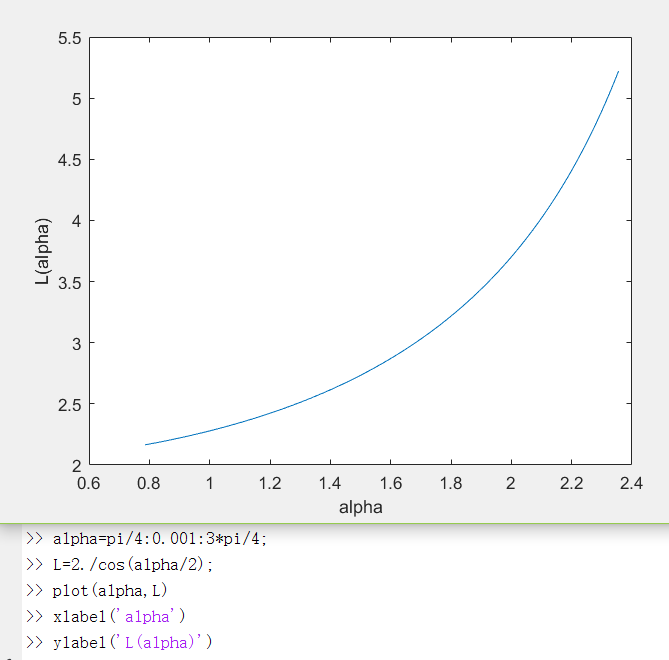
\includegraphics[width=6cm]{5.png}
\end{figure}
If $d$ is in color 1, then $c$ is in color 2, $b$ and $f$ have to be  in color 1, and therefore $f$ and $b$ are in the same color while they are connected together. So this graph is not bipartite. 

\subsection*{iii)}
\begin{figure}[H]
    \centering
    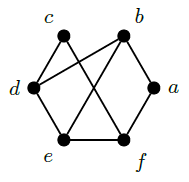
\includegraphics[width=6cm]{6.png}
\end{figure}
If $d$ is in color 1, then $c$ and $e$ are in color 2, $f$ have to be  in color 1, $a$ should be in color 2 and $b$ should be in color 1. Then $b$ and $d$ are in the same color while they are connected together. So this graph is not bipartite. 

\section*{Exercise 8.7}
\subsection*{i)}
\begin{figure}[H]
    \centering
    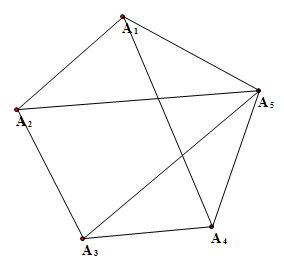
\includegraphics[width=8cm]{7.png}
\end{figure}

\subsection*{ii)}
\begin{figure}[H]
    \centering
    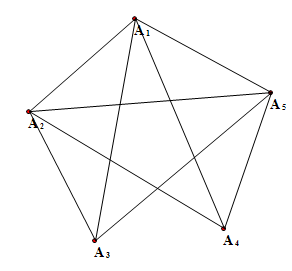
\includegraphics[width=8cm]{8.png}
\end{figure}
\subsection*{iii)}
\begin{figure}[H]
    \centering
    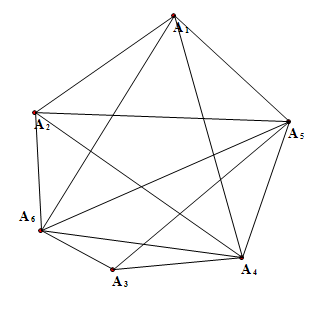
\includegraphics[width=8cm]{9.png}
\end{figure}




\end{document}
